\documentclass[../main.tex]{subfiles}
    
\begin{document}
The software is separated into modules according Figure \ref{table:specs}, where the
program is launched from ``main()''. The separation of modules of different
purpose allows for improving the software by focusing only one part of the
program. Some of the modules are just a wrapper for an API, which may be
implemented from scratch in the future. The purpose of the wrapper is to allow
the from-scratch-implementations, without rewriting the code for the module
using the API (e.g.\ without changing main to implement Text-to-Speech from
scratch).

\begin{figure}[ht!]
  \centering
  \caption{An UML of the software.\label{fig:uml}}
  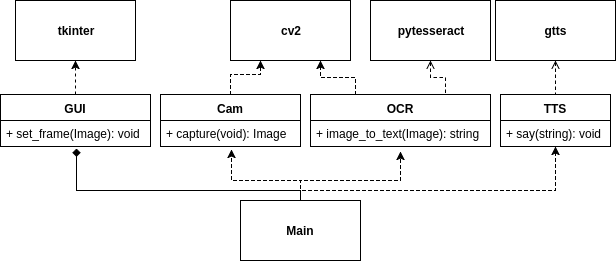
\includegraphics[width=1.0\textwidth]{uml}
\end{figure}

\subsection{GUI}
The graphical interface consists of a window that displays live camera feed and provides the user with the option to capture an image by pressing a button. Once an image been captured and analysed any text found will be returned and printed in a Terminal window. To be able to implement the camera, OpenCV is used. Its library provides methods to establish a connection between the GUI and the camera, that enables live camera feed to be displayed.

\subsection{Optical Character Recognition (OCR)}

OCR is the module that turns an image into characters. It uses OpenCV to pre-processes the image, before the image it is being passed to Tesseract, which recognises the characters. The pre-processing is meant to filter background noise to give more contrast to the text, which shall improve the performance of Tesseract. The pre-process applies a grayscale and adaptive gaussian threshold. (source) %(https://docs.opencv.org/3.3.1/d7/d4d/tutorial_py_thresholding.html).

\subsection{Text To Speech (TTS)}

TTS is the module that turns text (given from OCR) into speech. The module is a wrapper for gTTS, which is an interface for Google’s Text-To-Speech API \cite{github_gTTS}.

\end{document}
